\section{Energy and Electricity}
There is a mismatch between what many people believe uses most energy and reality.\\
Energy usage commonly\\
\textbf{overestimated}: warmwater, electronic equipment\\
\textbf{underestimated}: heating, personal car\\

\subsubsection{Energy in the industrial age}
Energy has been the fuel of the industrial age.
It has been a cheap driver of economic growth.
Measuring \cotwo in the atmosphere throughout hundreds of years we can see a big increase around 1800, likely caused by the invention of the steam engine. This development has continued and energy has become a major problem of the \textbf{late} industrial age.\\

\textbf{Energy problems}
\begin{itemize}
    \item Environmental issues (\cotwo etc.)
    \item Cost of acqusition
    \item Dependence on other countries (geopolitics)
    \item Renewable resources come with their own problems (unreliable, undispatchable)
\end{itemize}

\subsection{Energy}
Electricity $\subset$ Energy\\

Often energy usage leads to \cotwo emissions, which is one of the main modern day problems concerning energy.\\

The physical unit of energy is Joule. 1 J $=$ 1 Ws, the work required to produce one W of power for one second.
The sun yearly outputs $\sim 10^{13}$ ZJ.
Human society only need a tiny fraction of this energy which leads to a big engineering problem.
The world yearly energy consumption is $\sim 0.627$ ZJ, which corresponds to $\sim 2000$ J / person at any instant.
This number is higher in highly developed countries (Europe etc.).\\

What can we do with \textbf{1 Joule}
\begin{itemize}
    \item Lift an apple 1 meter
    \item Send $\sim$ 1 MB over WiFi
    \item Make a 2 second phonecall
    \item Drive a car 0.35 mm
\end{itemize}

Key idea of smart energy technology is that communication uses much less energy than transportation and heating.
We can save energy in these areas by using more ICT.

\subsubsection{Primary and Final Energy}
Total energy \textbf{consumption} (supply) is different than actual \textbf{end usage} due to energy loss.
Consider for example transforming coal into electricity.
In this process 60\% of the energy is lost.
This motivates a concept of \textbf{quality} of energy.
Heat is low-quality energy, electricity is high-quality energy.\\

Final energy can be seen as energy used on site, for example in a home.
In final energy electricity usage is comparable to other sources, but because electricity generation often require multiple units of lower quality sources it has a larger footprint in the primary energy consumption.\\

\begin{figure}
    \centering
    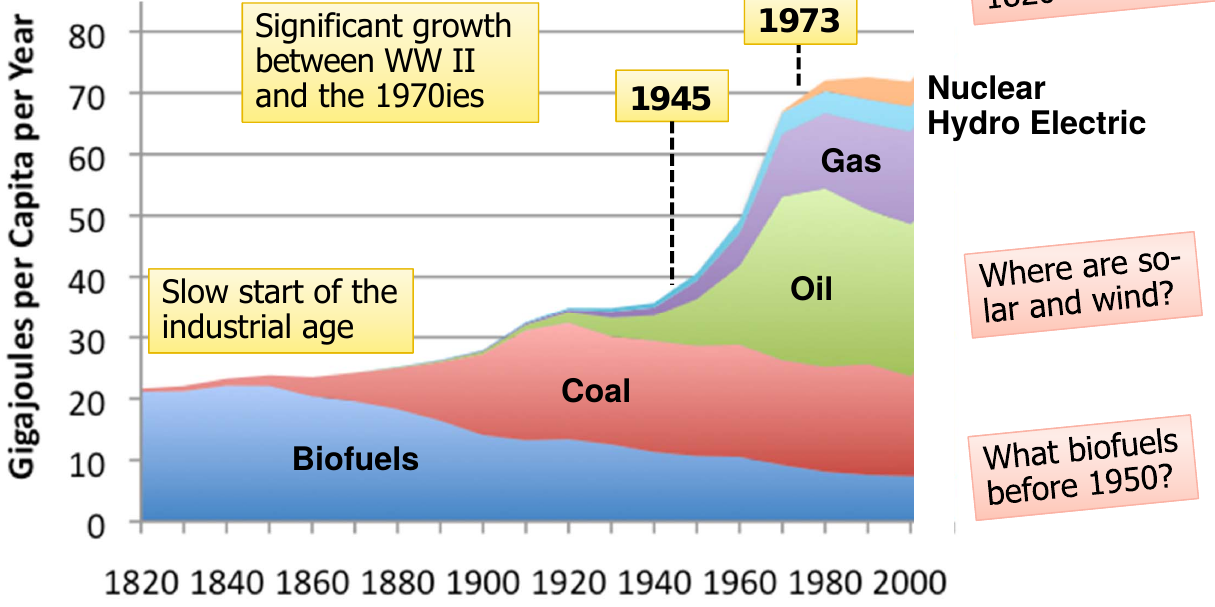
\includegraphics[width=0.7\linewidth]{primary_energy_consumption}
    \caption{Primary Energy Consumption per Capita}
    \label{fig:primary_energy}
\end{figure}

In figure \ref{fig:primary_energy} we can see trends in primary energy.
Note the decrease of biofuels, the rise and fall of oil, the increased usage of gas and the missing solar and wind power. It is clear that the total primary energy consumption has grown, but flattened out since 1973.\\

Since the 70s the primary energy consumption per capita in the US and Europe has stayed mostly the same.
Since 2000 we do however see a large increase in Asia and Africa.
This combined with a large population increase in these areas predict a future energy challenge.\\

There is a clear correlation between GDP (Gross Domestic Product) and primary energy consumption per capita. The increase of GDP in Asia and Africa also points towards a future energy consumption increase.

\subsubsection{Energy usage by types}
In 2016 only $\sim$ 9\% of energy used was estimated to come from renewable resources.
Less than 2\% of this was from so called new renewables (solar PV, wind etc.).
Changes in what types of resources is used is very slow due to long asset lifetimes.\\

\begin{figure}
    \centering
    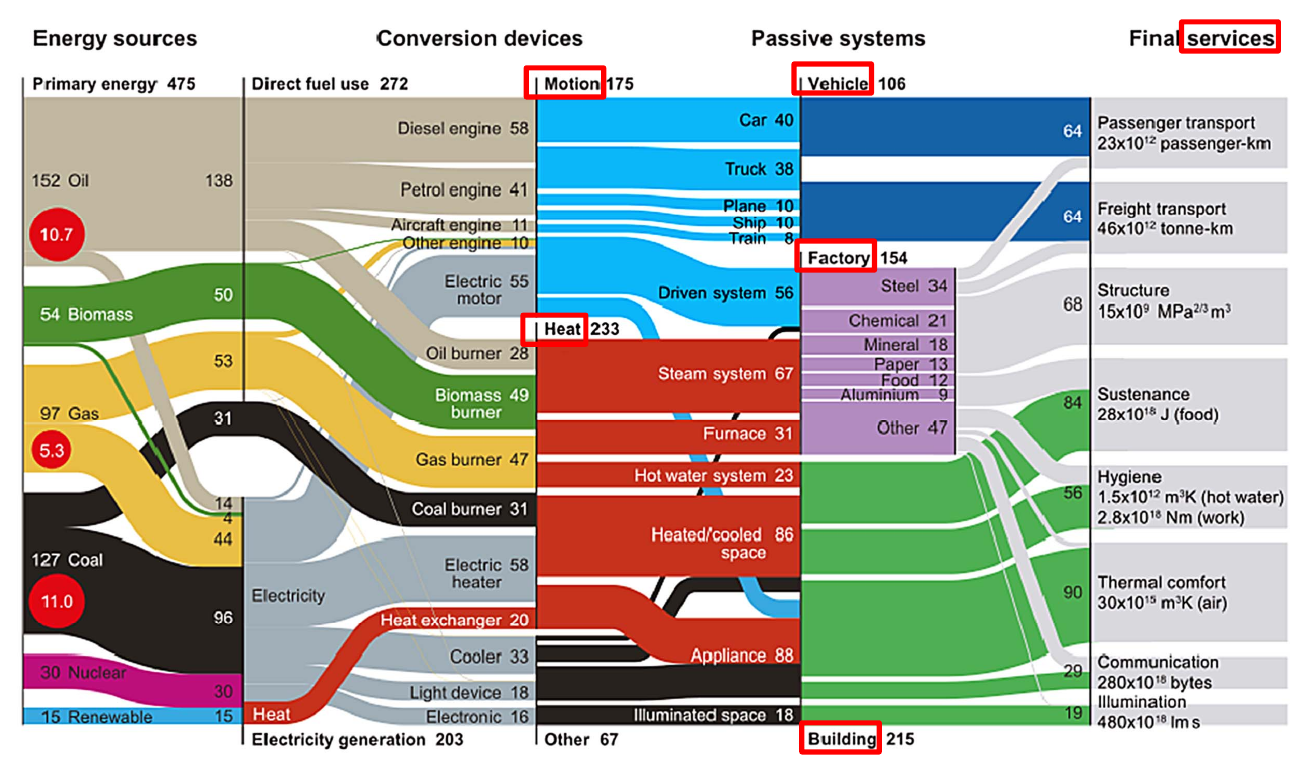
\includegraphics[width=\linewidth]{sankey_world}
    \caption{World energy flow 2005}
    \label{fig:sankey_world}
\end{figure}

Sankey diagrams visualize how energy transfers between processes.
They start in types of primary energy and ends in energy used in different sectors.
A sankey diagram for world energy flow 2005 can be seen in figure \ref{fig:sankey_world}.\\

In Switzerland the use of oil increased drastically up until the oil crisis in 1973.
Ater that the oil use has decreased and use of electricity and natural gas increased.

\subsubsection{Oil Crisis}
The 1973 oil crisis was a consequence of an oil embargo from Arab Petroleum Exporting Countries.
The reason for the embargo was related to US support of Israel.
During the oil crisis prizes for gasoline rose and rations were proclaimed in many countries. The crisis ended with the embargo in 1974, but the event impacted the future use of oil.

\subsubsection{Swiss Nuclear Phase Out}
Switzerland is currently committed to phasing out nuclear power.
This represents a big challenge since about 40\% of Swiss power comes from nuclear.
There are little opportunity to increase hydro power, so one discussed approach is to use more natural gas.
This is however controversial since it would carbonize Swiss electricity.

\subsection{Electricity Production}

\subsubsection{Swiss Hydro Energy}
Hydropower represents more than half of Swiss electricty production and will take up an even larger fraction as nuclear is phased out.
The electricity production from hydro has mostly stayed constant in the past 40 years.
Other renewables represent a very small fraction ($<$ 5\% in 2015).
Switzerland is in a very privileged situation when it comes to hydro power because of the landscape being filled with mountains and valleys.
This is very suitable for reservoir power stations where energy can be stored by pumping water to higher altitudes.
These power plants can be ramped up and down within minutes to adapt to changing energy demands.\\

In Switzerland the \cotwo emissions of electricity being consumed is 7 times higher than due to electricity being produced.
Generally Switzerland exports about as much electricity as is imported. It is worth noting that the electricity exported is clean and the electricity being imported is dirty (clean, dirty referring to greenhouse gas footprint).

\subsubsection{International Electricity Production}
The US relies mainly on fossile fuels for electricity production.
France mainly get its electricity from nuclear power.
Germany are very reliant on fossil fuels and have a similar struggle as Switzerland with facing out nuclear power.\\

Different countries use rather different mixes of primary resources.
Reasons for this are

\begin{itemize}
    \item geographical
    \item geological
    \item economical
    \item historical
    \item political.
\end{itemize}

In the EU the trends in electricity generation are
\begin{itemize}
    \item Declining use of oil.
    \item Large increase in windpower
    \item Large increase in use of biomass
    \item Increase in use of gas
\end{itemize}

On a global scale the electricity generation from renewables is largely dominated by hydro power.\\

It is predicted that electricty generation will increase with 80\% until 2035.
The prediction is that increased use of renewables will not compensate for this increase.
Even though we can expect renewable electricity generation to increase we will also see increased use of coal, gas and oil to compensate for the large total increase.
